% Définition du nom du chapitre
\chapter[Fine-scale automatic mapping of living \textit{Posidonia oceanica} seagrass beds with underwater photogrammetry]{Chapitre 3: Fine-scale automatic mapping of living \textit{Posidonia oceanica} seagrass beds with underwater photogrammetry} \label{chapitre3-herbiers}

\pagestyle{main}

%%%%%%%%%%%%%%%%%%%%%%%%%%%%%
%%% Figure cover chapitre %%%
%%%%%%%%%%%%%%%%%%%%%%%%%%%%%
\begin{tikzpicture}
  \def\ig{%
   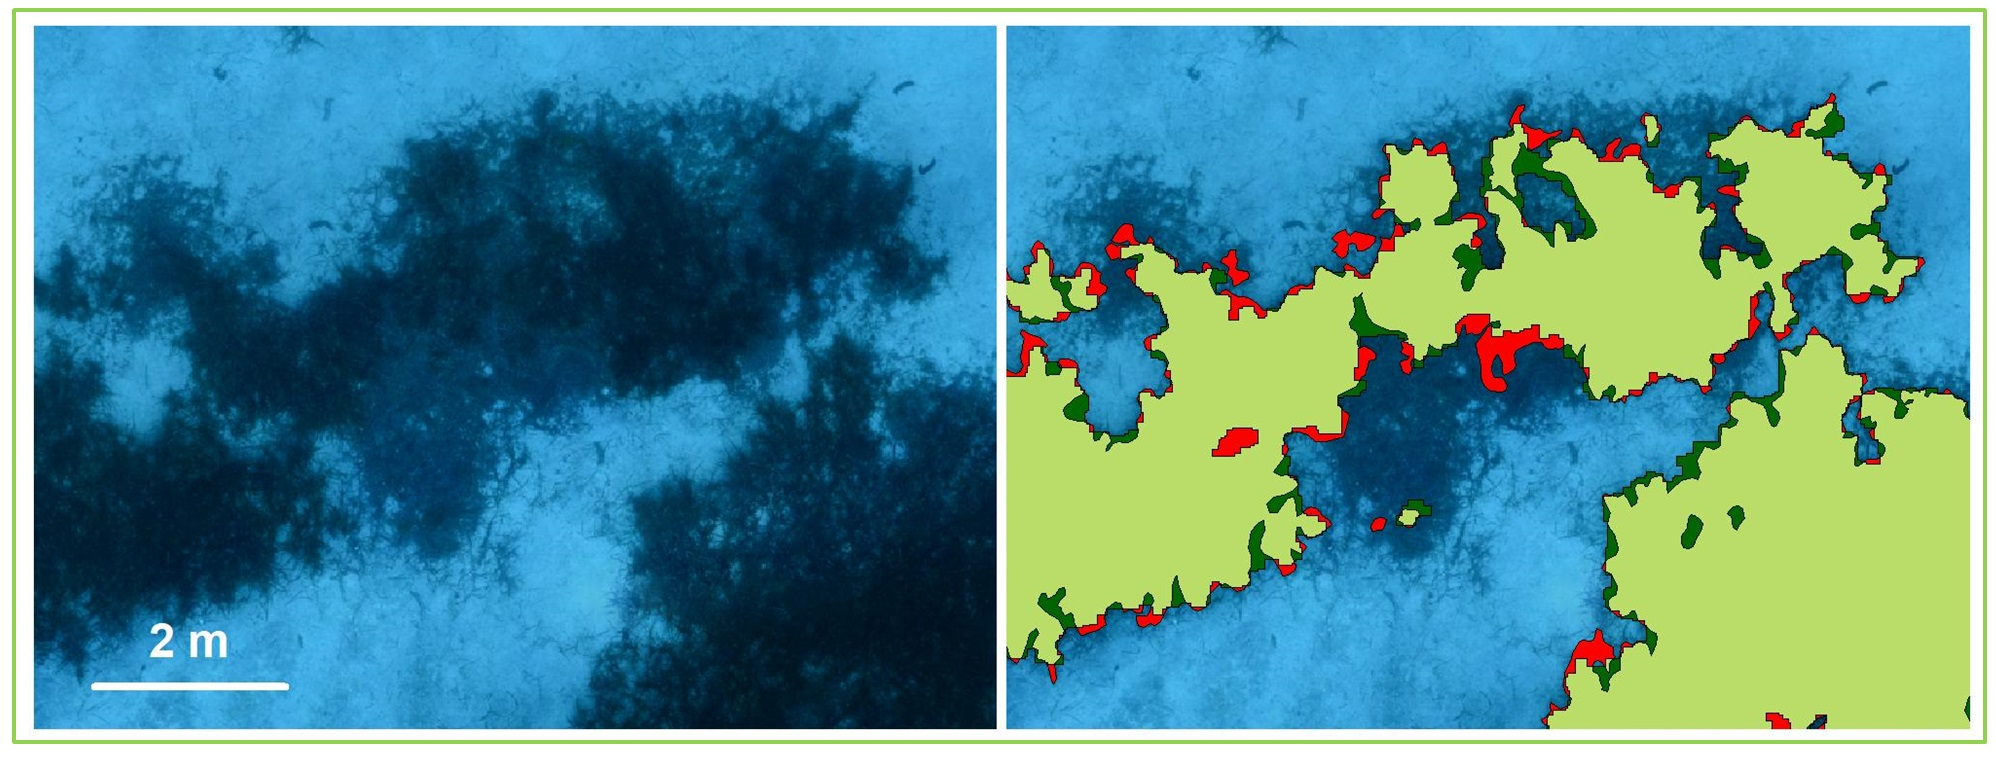
\includegraphics[width=\linewidth,keepaspectratio]{./5_chapitre3/cover.jpg}}
 \node [inner sep=0pt](mypicture) at (0,0) {\phantom{\ig}};
 \clip[rounded corners=5mm] ($(mypicture.south west)+(\bord,\bord)$) rectangle ($(mypicture.north east)-(\bord,\bord)$);
 \node[inner sep=0pt](mypicture) at (0,0) {\ig};
\end{tikzpicture}

% Bullet points du début de chapitre
\begin{center}
\begin{colbox}{resume}
  \vspace{-2pt}
{\color{textresume}\small
\begin{itemize}[leftmargin=0in]\itemsep3pt
\item \textbf{OBJECTIFS}~:
    \begin{itemize}
      \item Mise au point d'une \textbf{méthode de cartographie} automatique des herbiers de Posidonie par \textbf{photogrammétrie}~;
      \item \textbf{Application} de la méthode pour des suivis d'herbiers en limite inférieure~;
    \end{itemize}
\item \textbf{RESULTATS}~:
    \begin{itemize}
      \item La \textbf{précision}, le \textbf{taux de rappel} et le \textbf{F1-score} moyens sur 21 sites sont respectivement de \textbf{0.79, 0.91} et \textbf{0.84}~;
      \item La \textbf{profondeur}, le \textbf{type de substrat}, la \textbf{surface} de la zone d'étude ainsi que la \textbf{densité} de l'herbier n'ont pas d'influence significative sur la précision de la méthode~;
      \item Le niveau de \textbf{fragmentation} de l'herbier affecte significativement la qualité de la classification.
      \item L'application de la méthode pour le \textbf{suivi} de trois herbiers en limite inférieure montre \textbf{l'opérabilité} de la méthode et la \textbf{progression} des sites sur une période de 3 ans.
    \end{itemize}
\end{itemize}
}
\vspace{-2pt}
\end{colbox}
\end{center}

\clearpage

\noindent\textbf{Fine scale monitoring of living Posidonia oceanica}

% Auteurs
\noindent Guilhem Marre, Florian Holon, Sandra Luque, Pierre Boissery et Julie Deter

% NB sans indentation
\noindent\textit{En cours de révision dans...}

\noindent\textbf{Abstract}


\noindent\textbf{Keywords}

% Introduction
\section{Introduction}\label{chapitre3_1}

\newpage

% Material and methods
\section{Materials and methods}\label{chapitre3_2}

\subsection{Study sites}

\subsection{Data acquisition and processing}

\subsection{Workflow of the method}

\subsection{Assessment of classification accuracy}

\subsection{Influence of the site properties on classification performances}

\subsection{Monitoring the evolution of \textit{P. oceanica} meadows}

\newpage

% Results
\section{Results}\label{chapitre3_3}

\subsection{Method accuracy}

\subsection{Influence of the site properties on classification performances}

\subsection{Monitoring the evolution of \textit{P. oceanica} meadows}

\newpage

% Discussion
\section{Discussion}\label{chapitre3_4}


\subsection{Performances and limits of the methodology}


\subsection{Application of the methodology within a monitoring network}

\newpage
